Before we start with some hands-on data science, we think it is fundamental to ensure we are all on the same page on the Mathematics and Statistics we need throughout this course. But don't worry, it is nothing fancy. We, by no means, have the intent to \textit{formally} teach you any Mathematics. Instead, we just want to refresh some of the concepts we already know, but may have forgotten throughout the years.

\section{Mean, median, and standard deviation}

We would like to start with a good look at Fig. \ref{fig:boxplot}. This type of graphical representation is called a box-plot\footnote{The box-plot was created by John Wilder Tukey, the American Mathematician we talked about in Chapter 1.}. It shows the variation in miles per gallon (MPG) for cars with different numbers of cylinders\footnote{This data was extracted from the 1974 Motor Trend US magazine}. For now, let's focus only on cars with 4 cylinders. The black line just above 25 MPG is called median, i.e. the middle of the dataset. It indicates the point such that there is an equal probability of a MPG value falling above or below it. The top/bottom edges of the box indicate the upper and lower quartile, respectively. These quartiles tell us that there is only 25$\%$ chance a car with 4 cylinders will use more than 30 or less than 23 MPG. \textit{Did you realize that already 50$\%$ of our data lies within the box?} The horizontal lines above/below the box represent the maximum/minimum MPG values excluding outliers. Here, outliers are defined as MPG which appear less often than 10$\%$ of the cars with 4 cylinders, i.e. above 34 MPG or below 21 MPG.

\begin{figure}[h]
	\begin{center}
			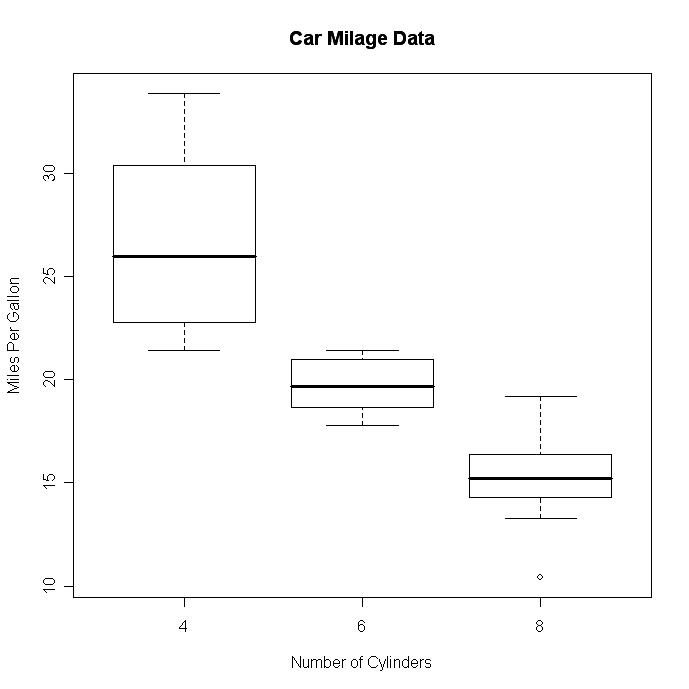
\includegraphics[scale=0.3]{Parts/basics/milleagech2}
	\end{center}
	\caption{Box-plot of miles per gallon by car cylinders. This data was extracted from the 1974 Motor Trend US magazine.}
	\label{fig:boxplot}
\end{figure} 

Note that the thick horizontal black lines inside the boxes represent the respective \textit{medians} for 4, 6 or 8 cylinders. Note that this value is different than the mean value. Here is why: the ``mean'' represents the ``average'' we all know. Simply sum up all the numbers and then divide them by the total number of occurrences. The ``median'' represents the ``middle'' of a ordered series of numbers. This is important because in practice we always find distributions which are highly skewed. In those cases, the median is more representative than the mean.

The mean or the median alone do not tell us the whole story about our data. We still have to understand the data \textit{distribution} and how the individual points are spread around the mean. To help us with that we will introduce the concept of standard deviation. In a nutshell, it represents by how much the individual samples differ from the mean. We depict it in Fig. \ref{fig:std}.

\begin{figure}[h]
	\begin{center}
			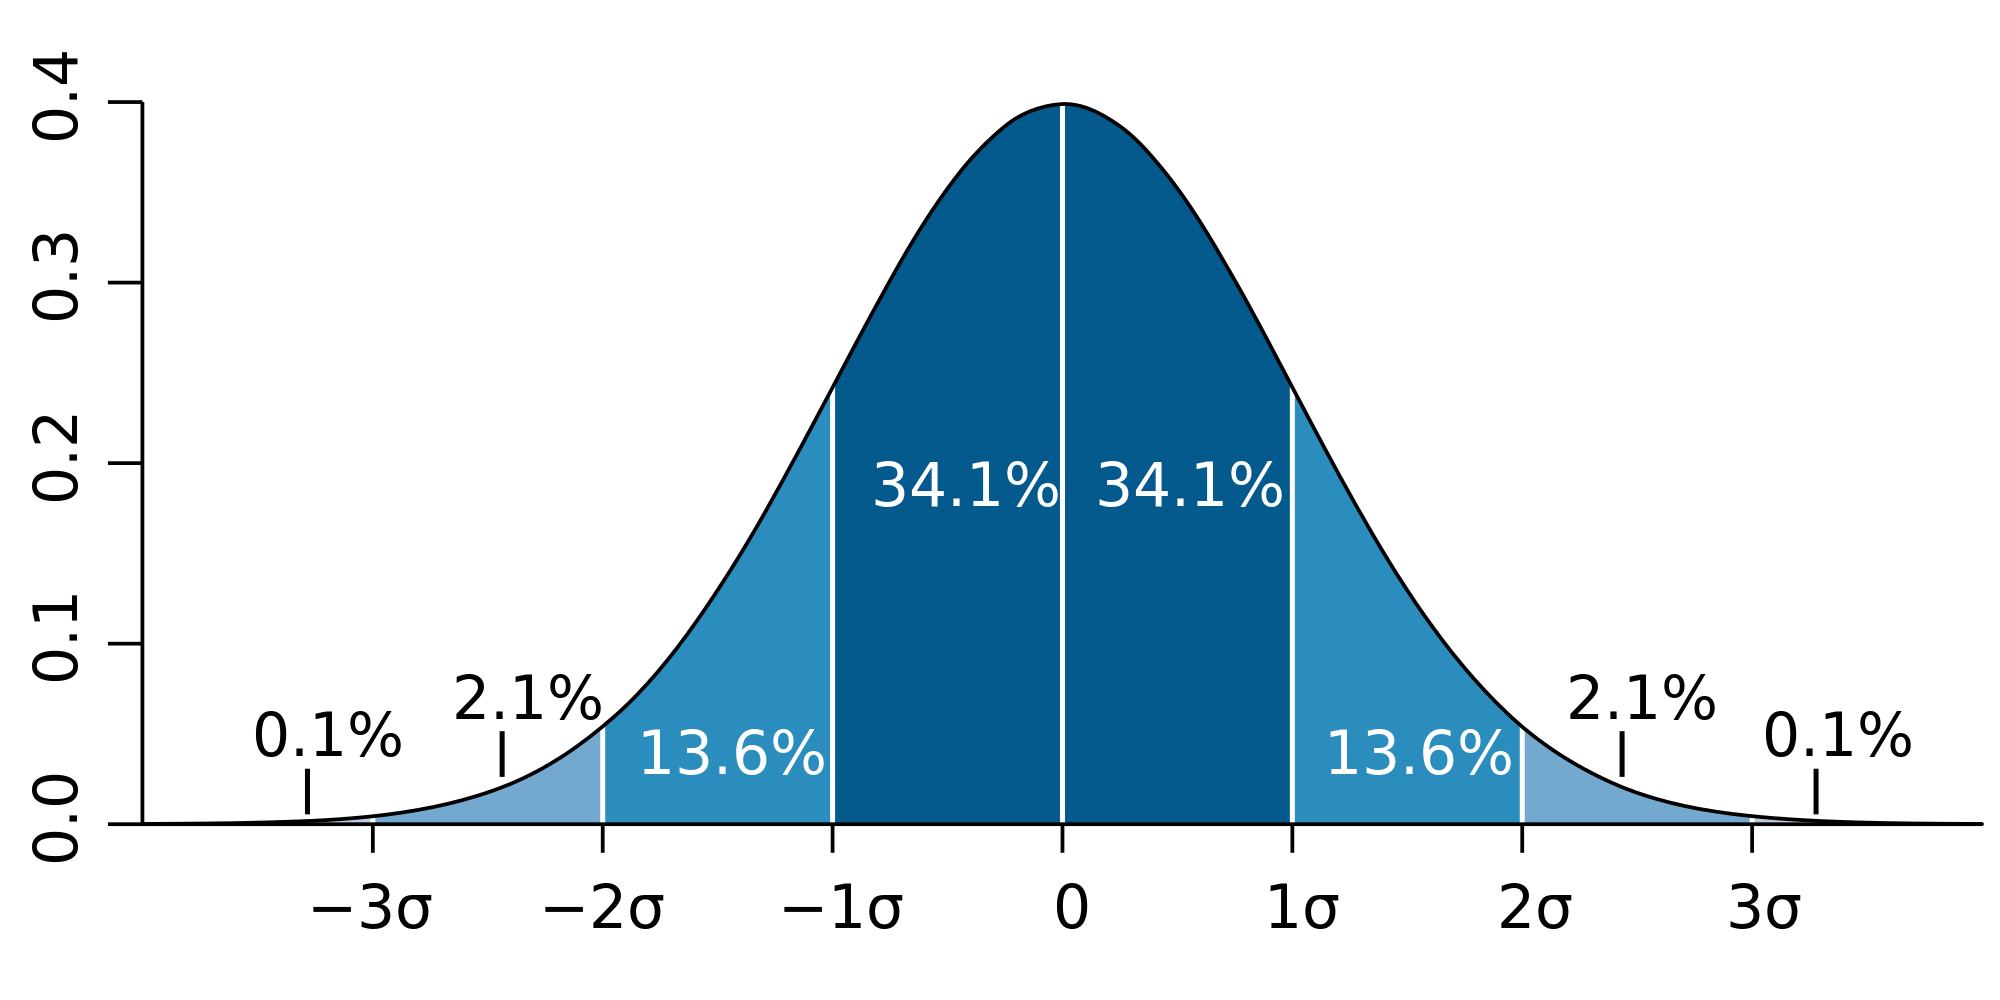
\includegraphics[scale=0.13]{Parts/basics/stdch2}
	\end{center}
	\caption{Normal distribution where each band accounts for $\pm$ 1 standard deviation}
	\label{fig:std}
\end{figure} 

\newpage

The standard deviation is a measure of the dispersion of your data. That means a small standard deviation indicates little dispersion around the average. In contrast, a high standard deviation indicates significant dispersion around the average. As shown in Fig. \ref{fig:std}, the width of one standard deviation ``covers'' roughly 68$\%$ of the data dispersion. That number increases to over 99$\%$ for three standard deviations.

\section{Interpreting a plot, tracing a linear fit, and understanding R$^2$}

Another important topic we want to talk is how to interpret plots. As we show in Chapter \ref{Commun} plots are a fundamental way to communicate your data-science results within your company. For now, we will focus on extracting some interesting information from Fig. \ref{fig:linR}. Later, we go in much greater detail on how to design plots and interpret such model results.

\begin{figure}[h]
	\begin{center}
			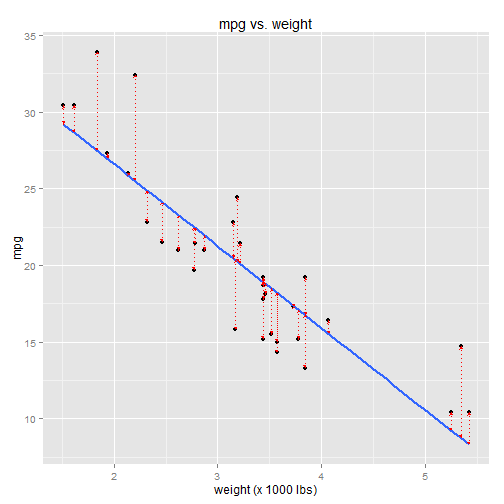
\includegraphics[scale=0.35]{Parts/basics/linregch2}
	\end{center}
	\caption{Miles per gallon versus the weight of the cars. The blue line draws a linear relation between MPG and the weight of the cars. The red dotted-lines represent the difference (residuum) between the linear fit and each data point. This data was extracted from the 1974 Motor Trend US magazine.}
	\label{fig:linR}
\end{figure} 

We observe a negative correlation between MPG and weight of the car. As the weight increases, MPG decreases. Note that this follows intuitively, since we expect heavier cars to use more fuel and therefore have lower MPG. The blue line represents a linear fit between the variables. The criterion to obtain the linear fit is to minimize the distance between the fit and the data points. This difference is called residuum (shown in red in Fig. \ref{fig:linR}). In Chapter \ref{numerics} we will cover the design of such simple numerical model in much greater detail. 

\newpage

For now let's assume we know how to implement such model - but how do we measure its performance? A simple way to achieve that is by calculating the so-called \textit{determination coefficient}, known as (R$^2$). R$^2$ is a metric that uses the residua information to determine if a linear fit is acceptable or not. It ranges from 0 to 1, where zero means no correlation between variables and 1 means a perfect fit. In the case shown in Fig. \ref{fig:linR} we find that $R^2=0.75$, indicating a good linear fit between MPG and weight of the car. In other words, the weight of the car can explain 75$\%$ of the MPG's variance. Generally speaking we define $R^2>0.5$ as acceptable. 
 
\section{Histograms}

The last topic we want to cover in this Chapter is histograms. A histogram is nothing more than a bar plot whose area represents the frequency of a given variable. In Fig. \ref{fig:histch2} we can visualize a histogram showing the frequency of the MPG variable:

\begin{figure}[h]
	\begin{center}
			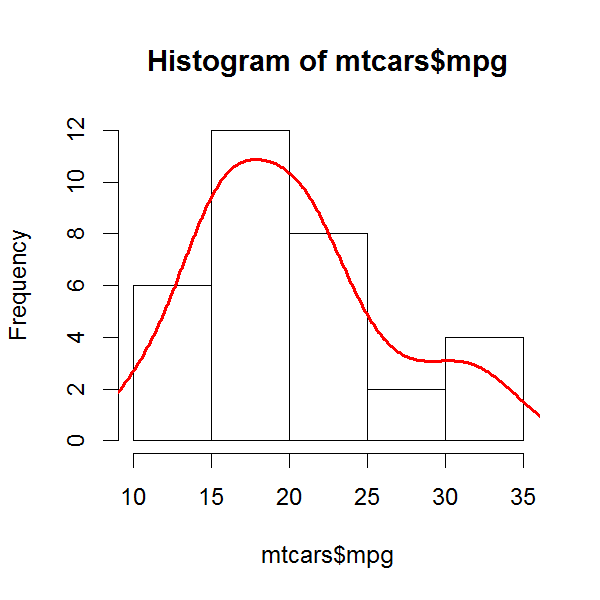
\includegraphics[scale=0.7]{Parts/basics/histch2}
	\end{center}
	\caption{Histogram showing the MPG frequency distribution. The red line emphasize its distribution. This data was extracted from the 1974 Motor Trend US magazine.}
	\label{fig:histch2}
\end{figure} 

\newpage

Note that the width of the bars represents the class interval. In our case every bar shows the frequency for an interval equal to 5 MPG. We can conclude from this plot that most cars have a MPG usage between 15 and 20 followed by 20-25 MPG (see also the red line). This plot also triggers many more questions, such as why is the frequency of cars using 30-35 MPG higher if compared to 25-30 MPG? It is not  possible to answer this question by only looking at this plot. The correct strategy is to combine a number of different analyses and plot more variables to understand this behaviour. We will exemplify that in Chapters \ref{harvesting} and \ref{numerics}.